\chapter{波动光学够用本}
\label{ch:03}

\section{效果}
\label{sec:ch03-effect}

读完本章，你应能：
\begin{enumerate}
  \item 用双光束干涉解释条纹强度如何随相位 $\varphi$（或光程差 $\OPD$/$\opd$）变化，并写出可见度 $V$ 的含义；
  \item 陈述相干长度的够用直觉：何时还能看见稳定干涉，何时条纹被「洗掉」；
  \item 把衍射极限、艾里斑与点扩散函数 $\PSF$（记 $h$）联系起来，说明分辨率与数值孔径 $\NA$、波长 $\wavelength$ 的折中；
  \item 在结构光场景中诊断：条纹对比度塌陷究竟更像离焦、衍射截止，还是光源相干/带宽问题。
\end{enumerate}

\section{原理}
\label{sec:ch03-principle}

\subsection{从几何光线到相位}

第~\ref{ch:01}~章的针孔与薄透镜回答「光线往哪走」。结构光与干涉测量还要问：两束光在像面某点的\textbf{相位差}是多少。单色平面波的相位沿传播积累；两路光程之差记为光程差 $\OPD$（亦常用 $\opd$），与相位的关系为
\begin{equation}
  \varphi = \frac{2\pi}{\wavelength}\,\opd
  \quad\text{（或}\ \varphi=\tfrac{2\pi}{\wavelength}\,\OPD\text{）}.
  \label{eq:ch03-phase-opd}
\end{equation}
记号锁定：$\wavelength$ 只表示波长；光学频率为 $\nuopt$（满足 $c=\wavelength\nuopt$ 在真空中）；焦距仍是 $f$，绝不用 $f$ 表示频率。

\subsection{双光束干涉与条纹}

设两束相干光在观察点的复振幅相加，平均强度（辐射度量语境下更接近辐照度时用 $E$，本章谈干涉条纹时沿用强度 $I$ 并注明）可写成
\begin{equation}
  I = I_1+I_2+2\sqrt{I_1 I_2}\,\lvert\gamma\rvert\cos\varphi,
  \label{eq:ch03-twobeam}
\end{equation}
其中 $\varphi$ 含几何相位与可能的初始相位；$\lvert\gamma\rvert$ 概括相干程度（完全相干时取 $1$ 的理想化）。若 $I_1=I_2=I_0/2$，则
\begin{equation}
  I = I_0\bigl(1+V\cos\varphi\bigr),
  \qquad
  V=\frac{I_{\max}-I_{\min}}{I_{\max}+I_{\min}}.
  \label{eq:ch03-visibility}
\end{equation}
$V$ 称为条纹可见度（对比度）。$V\to0$ 时条纹消失，相位无法从强度中稳健估计——这正是结构光解码失败的常见光学原因之一 \citep{HechtOptics,BornWolf}。

\begin{figure}[htbp]
  \centering
  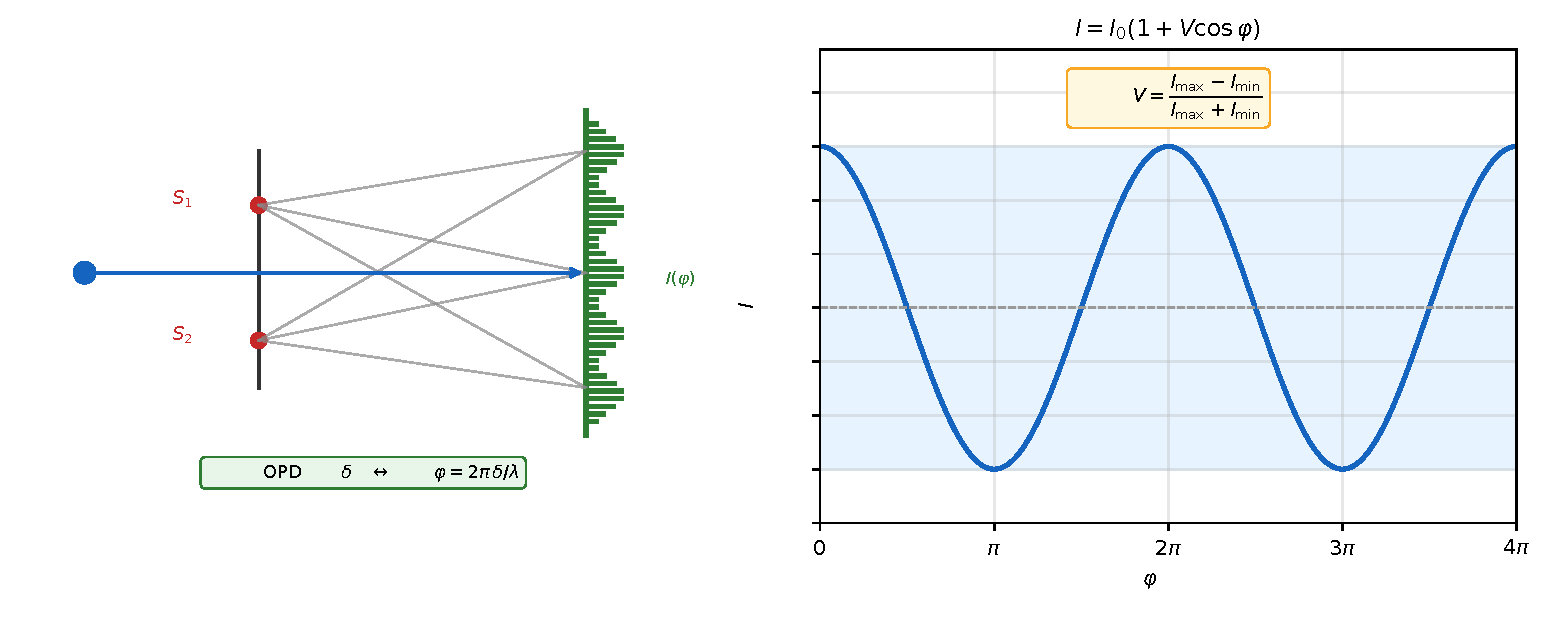
\includegraphics[width=0.95\textwidth]{fig-interference-twobeam.pdf}
  \caption{双光束干涉概念草图（非精确工程图）。左：双路到屏上形成条纹；右：强度随相位振荡，振幅由可见度 $V$ 决定。}
  \label{fig:ch03-interference}
\end{figure}

杨氏双缝给出空间条纹；分振幅干涉（薄膜、迈克尔逊等）给出随光程扫描的条纹。结构光投影仪把「已知空间相位编码」投到物体上，相机记录的是经表面反射/散射后的\textbf{调制度图案}；其可解码性首先要求 $V$ 足够大，其次才是算法。

\subsection{相干长度：够用直觉}

真实光源有频谱宽度。频谱越宽，不同频率成分的干涉条纹错位叠加，有效可见度随光程差增大而下降。相干长度 $\ell_c$ 可粗估为
\begin{equation}
  \ell_c \;\sim\; \frac{\wavelength^{2}}{\Delta\wavelength},
  \label{eq:ch03-coherence-length}
\end{equation}
其中 $\Delta\wavelength$ 为有效光谱宽度（数量级关系，精确定义依频谱形状）。当 $|\OPD|\ll\ell_c$ 时，干涉仍可清晰；当 $|\OPD|$ 接近或超过 $\ell_c$，条纹被冲刷。LED、滤波宽带源、激光的 $\ell_c$ 可差多个数量级：激光易得高 $V$，但也更易在粗糙面上产生散斑（第~\ref{ch:04}~章）。

对「投影正弦条纹 + 相机成像」的主动光测量：光源往往只需\textbf{时间/空间部分相干}到能在相机积分时间内保持稳定图案；并非处处需要实验室级长相干。但若你做的是真干涉测距或光谱敏感的外差，相干长度就变成硬约束。

\subsection{衍射、艾里斑与分辨率}

有限孔径使理想点物的像不再是几何点，而呈衍射图案。圆孔远场的艾里斑中，第一暗环角半径约为
\begin{equation}
  \theta \;\approx\; 1.22\,\frac{\wavelength}{D},
  \label{eq:ch03-airy}
\end{equation}
$D$ 为孔径。物镜侧常用数值孔径 $\NA=n\sin\alpha$；瑞利分辨距离量级为 $0.61\wavelength/\NA$（浸液时 $n>1$ 可缩小）。更大 $\NA$ 提高横向分辨率，同时往往\textbf{压缩景深}（与第~\ref{ch:01}~章 $Z_d$ 的权衡一致）。

\subsection{点扩散函数 $\PSF$ 与 $\MTF$}

线性空不变成像下，像是物与点扩散函数 $h$（即 $\PSF$）的卷积。离焦、像差、衍射都使 $h$ 展宽。其频域传递为光学传递函数；模即为调制传递函数 $\MTF$：空间频率越高，调制度保留越少 \citep{GoodmanFourierOptics}。因此：
\begin{itemize}
  \item 条纹空间频率越高，越容易被 $\MTF$ 杀掉对比度；
  \item 离焦使 $\MTF$ 更早截止，表现为「条纹发灰、相位方差爆」；
  \item 像素采样还需满足奈奎斯特：光学截止与采样截止共同限制可用频率。
\end{itemize}

\begin{figure}[htbp]
  \centering
  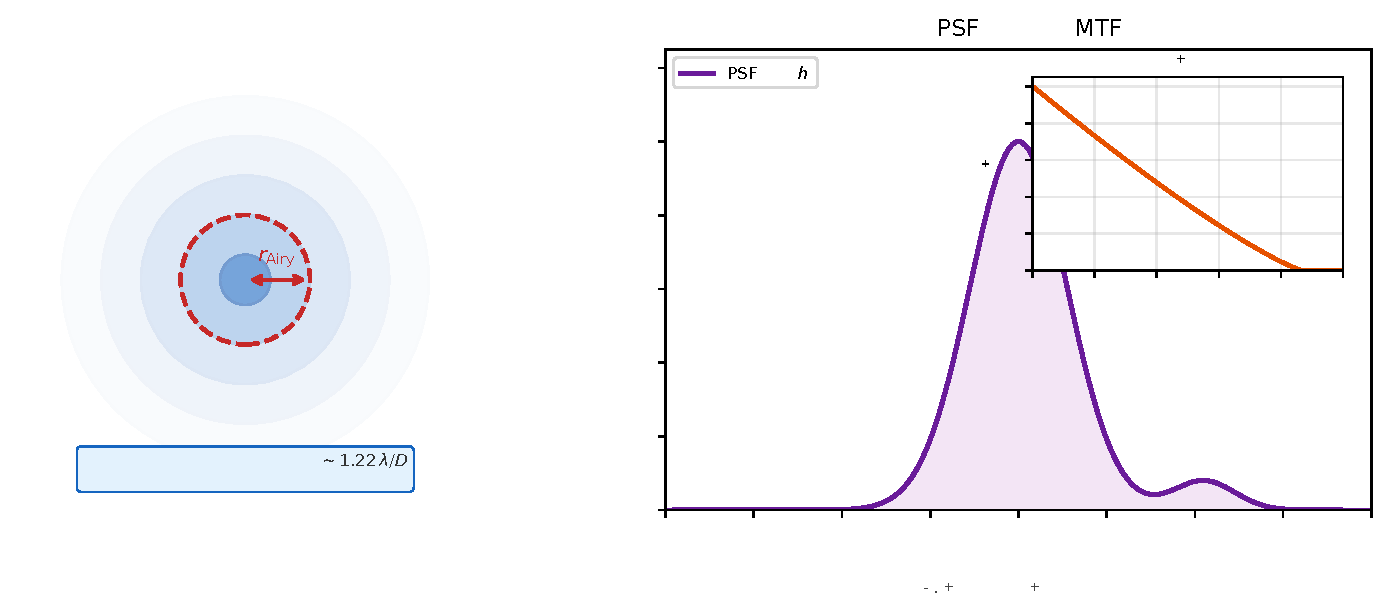
\includegraphics[width=0.95\textwidth]{fig-diffraction-psf.pdf}
  \caption{衍射极限艾里斑与 $\PSF$/$\MTF$ 概念草图（非精确工程图）。高频调制度先丢失，直接威胁细条纹与细纹理。}
  \label{fig:ch03-psf}
\end{figure}

\subsection{与重建分辨率的对接}

深度或形状分辨率往往\textbf{不是}「艾里斑直径直接写在点云上」。结构光里，相位估计精度大致随 $V$ 与 $\SNR$ 改善；三角测量再把像面误差放大为 $\delta Z$（第~\ref{ch:02}~章量级关系）。衍射与离焦同时抬高有效定位误差并降低 $V$，二者叠加。细纹理立体匹配同样吃 $\MTF$：纹理频谱落在截止外就无法匹配。

相位展开与解缠算法（如 \cite{GhigliaPritt1998}）假定条纹可辨；光学上已经 $V\approx0$ 的区域，再强的解缠也只是在噪声上作图。


\subsection{空间频率：条纹要落在系统通带内}

把投影条纹近似为像面上的余弦图案，其空间频率为 $\xi$（线对/毫米或周期/像素）。只有当 $\xi$ 落在光学 $\MTF$ 与传感器采样通带的交集内，调制度才以可见的 $V$ 到达解码器。提高 $\xi$ 本意是加密相位缠绕、提高深度灵敏度，但一旦越过截止，$V$ 崩溃，灵敏度反而变差。多频结构光的「低频保展开、高频提精度」正是在通带与解缠之间做调度：低频更耐离焦与衍射衰减。

采样侧：若每条纹周期少于约 $2$--$3$ 像素（再计非线性与噪声，实务常留更多余量），离散化本身就损 $V$。光学模糊核宽度 $\sigma_{h}$ 与条纹周期 $\Lambda$ 之比 $\sigma_{h}/\Lambda$ 是一个好用的无量纲诊断：比值增大时，先降频或先收锐对焦，而不是先改 CUDA 里的解缠参数。

\subsection{时间积分与振动}

相机曝光时间 $\tau$ 内若光程差或条纹相位因振动漂移 $\Delta\varphi(\tau)$，等价于对 $\cos\varphi$ 做时间平均，有效 $V$ 再乘一个衰减因子。手持口内扫描的微颤、投影风扇、地板振动，都会在高倍率、长相干架构里变成可见度杀手。短曝光提高瞬时锐度，但掉 $\SNR$（第~\ref{ch:05}~章）；脉冲照明与全局快门是光学–电子协同手段。

\section{限度}
\label{sec:ch03-limits}

\begin{itemize}
  \item 式~\eqref{eq:ch03-twobeam}--\eqref{eq:ch03-airy} 是标量、旁轴、够用模型；矢量偏振、严格电磁散射见深入教材 \citep{BornWolf}。
  \item 相干长度公式为数量级；LED 光谱非矩形时需用相干函数更细致描述。
  \item 「衍射极限」不保证系统达到该极限：像差、抖动、传感器采样常先成为瓶颈。
  \item 本章不展开完整傅里叶光学推导；需要传递函数设计时读 \cite{GoodmanFourierOptics}。
\end{itemize}

\section{对象}
\label{sec:ch03-object}

\textbf{结构光条纹对比度。} 正弦条纹投到牙面后相机所见 $V$ 不足：先分清——(1) 整体离焦/$Z_d$ 不够 → $\PSF$ 展宽、$\MTF$ 下降；(2) 条纹频率相对孔径与像素过高 → 衍射+采样截止；(3) 光源有效 $\Delta\wavelength$ 大且两路 $\OPD$ 大 → 相干冲刷（真干涉架构更常见）。提高投影亮度只改善光子 $\SNR$，\textbf{不}自动修复截止频率以外的调制度。

\textbf{离焦模糊。} 沟窝相对对焦面偏移时，局部 $V(u,v)$ 塌陷，相位图呈斑驳；点云在高频形貌处空洞。处置：收光圈换 $Z_d$（付 $\SNR$ 代价）、分层对焦，或降低条纹频率并改用多频策略。

\textbf{衍射对细纹理的限度。} 极细釉质裂纹或加工刀痕，其空间频率可能落在系统 $\MTF$ 之外：立体匹配失锁、结构光边缘相位偏置。这是物理分辨率预算，不是单纯「再训一个网络」能取消的。


\textbf{细条纹选型检查表。} 上线新条纹频率前，固定工作距与光圈，拍摄平面漫射靶：测量像面条纹周期（像素）与调制幅度；把频率逐步提高直到 $V$ 掉到预设阈值（例如低于 $0.3$），该频率即通带边缘。产品条纹应离边缘留裕量，因为牙面离焦与场曲还会再吃掉 $\MTF$。

\section*{本章收束}
干涉给出 $\varphi$ 与 $V$，相干长度约束何时有条纹，衍射与 $\PSF$/$\MTF$ 约束细条纹能否通过。结构光对比度问题应先问通带与离焦，再问算法。偏振与散斑将在第~\ref{ch:04}~章展开；通量与 $\SNR$ 在第~\ref{ch:05}~章展开。

\section{习题}
\label{sec:ch03-exercises}

\begin{enumerate}
  \item \textbf{（概念）} 为何条纹可见度 $V\to0$ 时，相位 $\varphi$ 难以从单像素强度估计？与「图像整体仍然很亮」是否矛盾？
  \item \textbf{（计算）} 两束等强完全相干，$I_0=100$（相对单位），$V=1$，$\varphi=\pi/2$。求 $I$。若 $V$ 降为 $0.2$ 而其余不变，$I$ 如何变？
  \item \textbf{（计算）} 中心波长 $\wavelength=550\,\mathrm{nm}$，有效 $\Delta\wavelength=20\,\mathrm{nm}$。粗估相干长度 $\ell_c$。若系统 $\OPD=0.5\,\mathrm{mm}$，条纹是否容易被冲刷？
  \item \textbf{（计算）} 孔径 $D=4\,\mathrm{mm}$，$\wavelength=550\,\mathrm{nm}$。用式~\eqref{eq:ch03-airy} 估角半径 $\theta$（弧度）。若像距约 $20\,\mathrm{mm}$，艾里斑半径量级（毫米）大约多少？
  \item \textbf{（重建场景）} 提高投影条纹频率后，中心对比度尚可、视场边缘条纹几乎消失。更可能是畸变模型错误，还是边缘 $\MTF$/相对孔径问题？给出检查顺序。
  \item \textbf{（重建场景）} 口内扫描沟底相位噪声大、牙尖正常。用 $Z_d$、$\PSF$、$V$ 写四步诊断。
  \item \textbf{（综合）} 激光照明 $V$ 很高但点云出现颗粒状抖动；LED 照明更平滑但对比度略低。这分别指向哪类波动/相干现象？（散斑细节见第~\ref{ch:04}~章。）
\end{enumerate}

\section{习题讲解}
\label{sec:ch03-solutions}

\begin{enumerate}
  \item $I=I_0(1+V\cos\varphi)$ 对 $\varphi$ 的灵敏度正比于 $V$。$V\to0$ 时 $I$ 对 $\varphi$ 几乎不变，无法反演。可以整体很亮（$I_0$ 大）但毫无调制，二者不矛盾。
  \item $I=I_0(1+V\cos\varphi)=100(1+1\cdot0)=100$。$V=0.2$ 时仍为 $100$（因 $\cos\pi/2=0$）。可见度改变的是极值差，不改变该相位点的瞬时 $I$；估计方差仍会因 $V$ 下降而变差。
  \item $\ell_c\sim\wavelength^{2}/\Delta\wavelength=(550\times10^{-9})^{2}/(20\times10^{-9})\approx15\,\mu\mathrm{m}$。$\OPD=0.5\,\mathrm{mm}\gg15\,\mu\mathrm{m}$，真干涉条纹极易被冲刷。普通投影纹理成像不依赖如此大的相干光程差。
  \item $\theta\approx1.22\times550\times10^{-9}/4\times10^{-3}\approx1.68\times10^{-4}\,\mathrm{rad}$。线半径 $\sim\theta s'\approx1.68\times10^{-4}\times20\approx3.4\,\mu\mathrm{m}$ 量级（概念估算）。
  \item 更优先查边缘照度、斜光束与局部离焦导致的 $\MTF$ 下降，以及相对孔径；畸变造成几何弯曲但不必先「消灭对比度」。顺序：看原图边缘 $V(u,v)$ → 查对焦场曲 → 再查曝光与投影均匀性 → 最后才怀疑纯几何标定。
  \item (1) 沟底是否超出 $Z_d$；(2) 局部 $\PSF$ 是否明显宽于牙尖；(3) 条纹局部 $V$ 是否塌；(4) 再查运动模糊与湿润高反（光度/偏振）。先光学后算法。
  \item 激光：高相干 → 粗糙面散斑，相位/匹配出现颗粒噪声。LED：较短相干、较少散斑，但可能较低 $V$ 或较低通量。需在散斑与对比度之间做光源选型折中。
\end{enumerate}
